\section{Filtrovanie zašumeného signálu}
\label{sec:ziskavanieRychlosti}

Ako bolo spomenuté v~predchádzajúcej kapitole, rýchlosti kolies sa dajú získať z~enkóderov. Tieto dáta sa posielajú v~správe, ktorá pripomína JSON formát.
Z~týchto vzoriek poslaných robotom nevieme priamo vypočítať polohu. Musíme si tieto dáta premeniť z~impulzov za~sekundu \(\frac{1}{s}\) na~metre
za~sekundu \(\frac{m}{s}\). Tento prevod nebude jednoznačný, pretože každý z~enkóderov posiela dáta inak zašumené. Preto~je potrebné zistiť, ako sa zmení
rýchlosť pri~zmene impulzov za~sekundu. Tento prevod (sklon prelozenej linearnej regresie cez~namerané data) je možné získať z~merania, kde~po~nastavení
rýchlostí zoberieme veľa dát z~enkóderov a~zistíme, ako sa zmení rýchlosť pri~zmene impulzov za~sekundu.

Prvý nápad na~získanie čo najlepšej prevodovej charakteristiky bolo cez~všetky dáta položiť lineárnu regresiu. To~sa ukázalo ako zlé riešenie, lebo dáta,
ktoré dostávame majú veľmi veľký rozptyl. Jednou z~nasledujúcich úvah bolo spraviť kĺzavý priemer. Toto riešenie malo tiež svoje chyby a~to~v~tom, že~zmeny
zaznamenaných impulzov za~sekundu sa zmenili v~závislosti od~rýchlosti a~smeru Obr.~\ref{fig:rw_lw_nf}. V~tomto bode sme vyskúšali počítať odometriu
z~obdržaných dát. Táto implementácia bola veľmi nepresná. Zároveň nám tento pokus potvrdil, že~potrebujeme filtrovať dáta, ktoré dostávame
od~robota, a~ktoré reprezentujú jeho rýchlosť v~impulzoch. Výsledky pokusu, kde~sme zisťovali prevodovú charakteristiku z~impulzov za~sekundu na~rýchlosť
v~SI jednotkách nájdeme na~nasledovných grafoch.

\begin{figure}[!htbp]
	\begin{subfigure}{0.5\textwidth}
		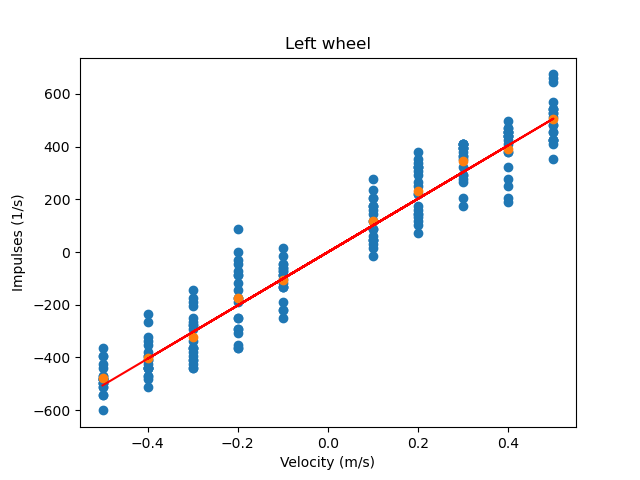
\includegraphics[width=\textwidth]{img/lw_nf.png}
	\end{subfigure}
	\hfill
	\begin{subfigure}{0.5\textwidth}
		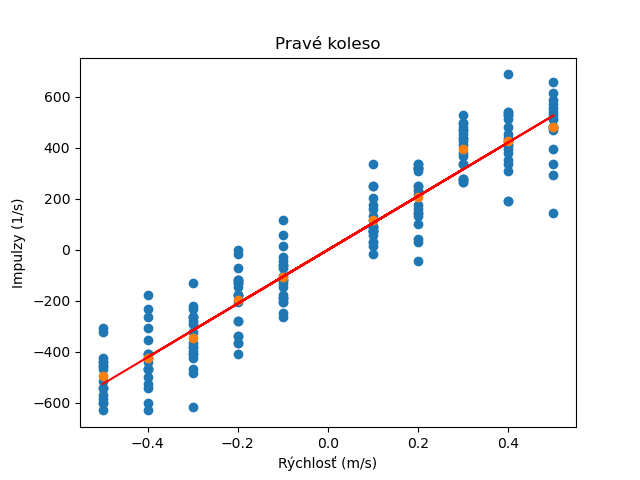
\includegraphics[width=\textwidth]{img/rw_nf.png}
	\end{subfigure}
	\caption{Získanie prevodu z~impulzov na~rýchlosť v~SI jednotkách.}
	\label{fig:rw_lw_nf}
\end{figure}

Ako prvú vec sme si vykreslili všetky \textbf{nazbierané dáta}. Tie sú~zobrazené \textbf{modrou} farbou. Cez~ne
sme spravili \textbf{lineárnu regresiu}. Je zobrazená ako \textbf{červená} úsečka. Z~nazbieraných dát sme si
nakoniec spravili priemer, aby sme videli, ako presne aproximuje nami vypočítaná lineárna regresia priemer
nazbieraných dát. \textbf{Priemery} jednotlivých rýchlostí sú~zobrazené ako \textbf{oranžové} body.
Keď sme cez~tieto dáta polozili priamku lineárnej regresie dostali sme sklon prevodu ľavého enkóderu. Jeho
hodnota je \textbf{1012,53636364}. Pre~pravý enkóder to~je hodnota \textbf{1053,67588345}. Tento parameter
môžeme použiť v~predpočítavaní nastavenej rýchlosti robota.

Môžeme si všimnúť, že~vypočítané priemery takmer presne ležia na~vypočítanej lineárnej aproximácie. Problémom je, ako už~bolo spomenuté, že~dáta,
ktoré dostávame od~robota sú~veľmi zašumené. Preto~z~nich nevieme priamo počítať polohu robota. Na~zobrazenie veľkosti odchýlky sme spravili
meranie. Nechali sme robot aby prešiel dráhu štvorca so~stranou dlhou 1 meter a~rýchlosťou 0,5 \(\frac{m}{s}\). Výsledok bol veľmi nepresný.
Metrom sme si odmerali jeho \textit{x}-ovú a~\textit{y}-ovú súradnicu s~počiatkom v~bode, kde~sme na~robote spustili náš ovládač. Jeho skutočná
poloha bola v~bode~(-0,3m,~0m). Čo~nám ale~vypočítala odometriu je, že~sa robot nachádzal 4 metre od~počiatku súradnicového systému.

\subsection{Zisťovanie parametru \(\alpha\)}

Implementovali sme si preto~dolnopriepustný kvadraticky filter. Fungovanie tohto filtra spočíva v~skombinovaní nového vstupného parametra a~starého parametra
uloženého vo~filtri v~danom pomere. Tento pomer je daný parametrom \textbf{alpha} $\alpha$.

\begin{equation}
	stavFiltra = \alpha * stavFiltra + (1 - \alpha) * nováVzorka
	\label{eq:stateOfFilter}
\end{equation}

Jeho parameter $\alpha$ sme získali viacerými meraniami. Začali sme najsilnejším filtrom s~hodnotou $\alpha$ rovnou  0,9.

\begin{figure}[!htbp]
	\begin{subfigure}{0.5\textwidth}
		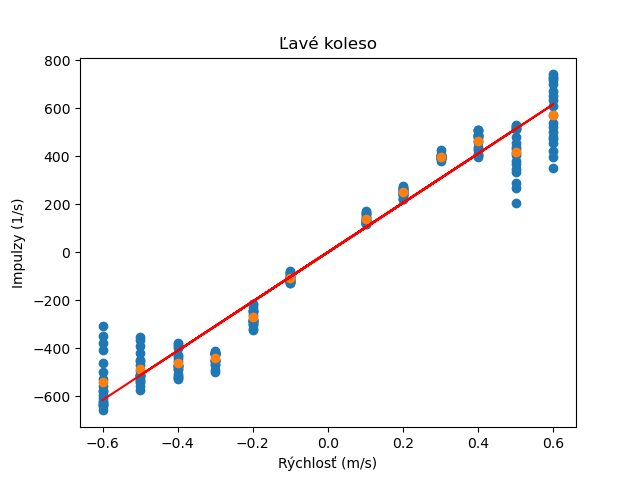
\includegraphics[width=\textwidth]{img/lw_09250.png}
	\end{subfigure}
	\hfill
	\begin{subfigure}{0.5\textwidth}
		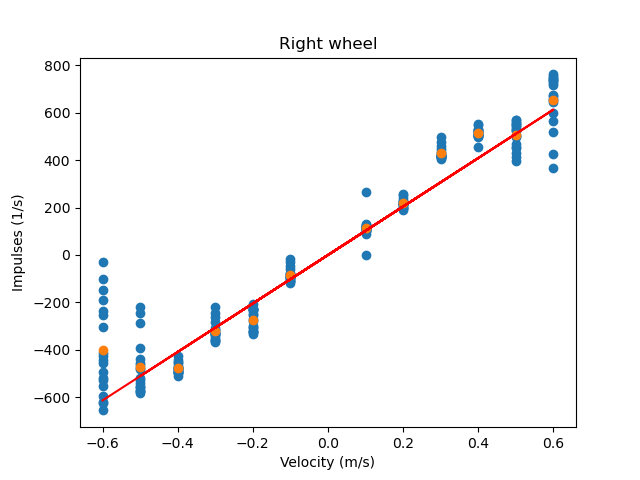
\includegraphics[width=\textwidth]{img/rw_09250.png}
	\end{subfigure}
	\caption{Získanie prevodu z~impulzov na~rýchlosť v~SI jednotkách. $\alpha$ = 0,9.}
	\label{fig:rw_lw_09250}
\end{figure}

Ako môžeme vidieť na~obrázkoch Obr.~\ref{fig:rw_lw_09250} a~Obr.~\ref{fig:rw_lw_nf} aplikácia filtra výrazne pomohla proti~šumu signálu.
Problémom pri~silnom filtri je to, že~ak~na~začiatku merania dostaneme zlú hodnotu, tak~sa táto hodnota ťažko mení na~správnu. Tento
efekt si môžeme všimnúť skoro pri~každej meranej rýchlosti. Najviditeľnejší dopad môžeme vidieť pri~pravom kolese
na~Obr.~\ref{fig:rw_lw_09250} pri~rýchlosti -0,6 $\frac{m}{s}$. Tento problém sme riešili postupným menením parametra filtru.
Aby sme predišli veľkému množstvu meraní, tak~sme použili metódy binárneho vyhľadávania. V~tomto prípade sme začali s~veľkou hodnotou
a~postupne sme skákali do~stredu nášho intervalu. Pre~toto meranie nám vysie koeficient sklonu lineárnej aproximácie
pre~ľavý enkóder \textbf{1028,04222094} a~pre~pravý nám vyšiel \textbf{1021,46905726} tento sklon. Kvôli vyššie spomenutým
dôvodom sme si ako ďalšiu hodnotu zvolili alphu $\alpha$ rovnú 0,7.

\begin{figure}[!htbp]
	\begin{subfigure}{0.5\textwidth}
		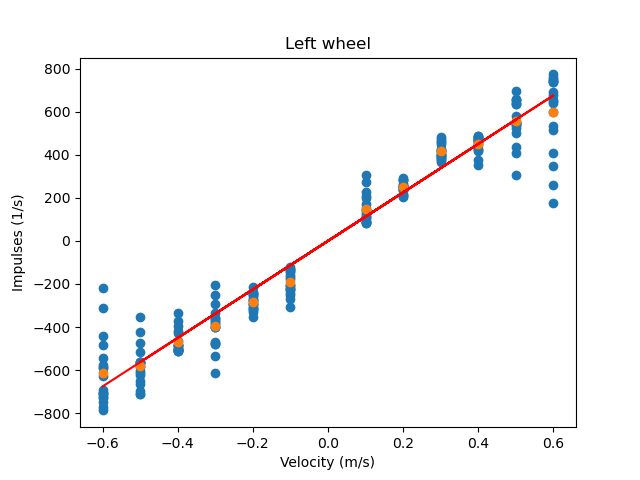
\includegraphics[width=\textwidth]{img/lw_07250.png}
	\end{subfigure}
	\hfill
	\begin{subfigure}{0.5\textwidth}
		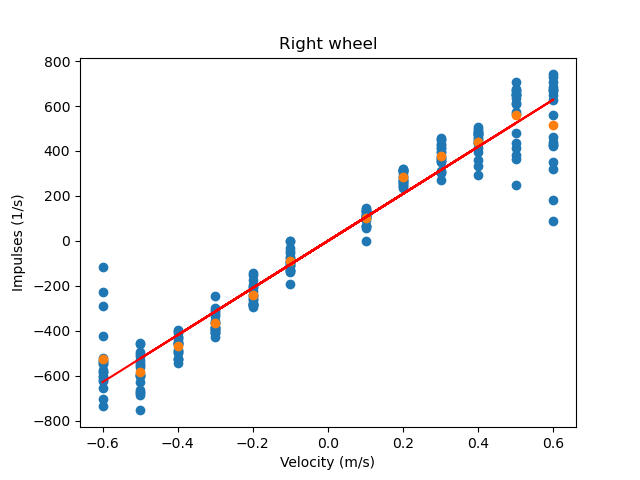
\includegraphics[width=\textwidth]{img/rw_07250.png}
	\end{subfigure}
	\caption{Získanie prevodu z~impulzov na~rýchlosť v~SI jednotkách. $\alpha$ = 0,7.}
	\label{fig:rw_lw_07250}
\end{figure}

Pri~použití koeficientu $\alpha$ s~hodnotou 0,7 (Obr.~\ref{fig:rw_lw_07250}) sme zistili, že~sa hodnoty rýchlosti aj~pri~aplikácii
filtra výrazne menili. Ustálené hodnoty zobrazené oranžovou farbou sú~podobne ako pri~meraní s~filtrom s~alphou $\alpha$
rovnou 0,9 mimo lineárnej regresie. Tá má sklon pre~ľavý enkóder \textbf{1126,16252169} a~pre~pravý enkóder to~je
\textbf{1048,61769809}. Neprekrytie priemeru a~aproximácie je zapríčinené iným dôvodom ako pri~silnejšom filtri. Pokým
pri~silnejšom filtri sme dostali zlú začiatočnú hodnotu, tak~už~bolo zložité ju zmeniť. Pri~slabšom filtri, ak~dostávame
rozdielne vstupné hodnoty tak~sa výstupná hodnota filtra ľahko mení. To~má za~dôsledok posun priemeru vstupných hodnôt.
Tento efekt sa dá odstrániť zosilnením filtra, čiže zväčšením koeficientu alpha $\alpha$. Spravili sme preto~ďalšie meranie,
kde~sme použili hodnotu $\alpha$ rovnou 0,75.

\begin{figure}[!htbp]
	\begin{subfigure}{0.5\textwidth}
		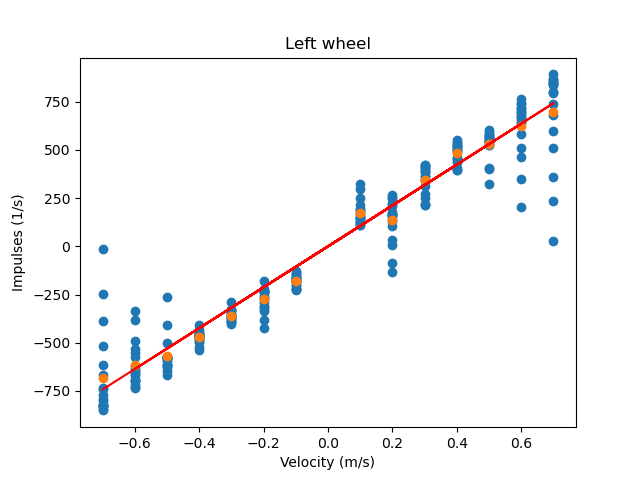
\includegraphics[width=\textwidth]{img/lw_075250.png}
	\end{subfigure}
	\hfill
	\begin{subfigure}{0.5\textwidth}
		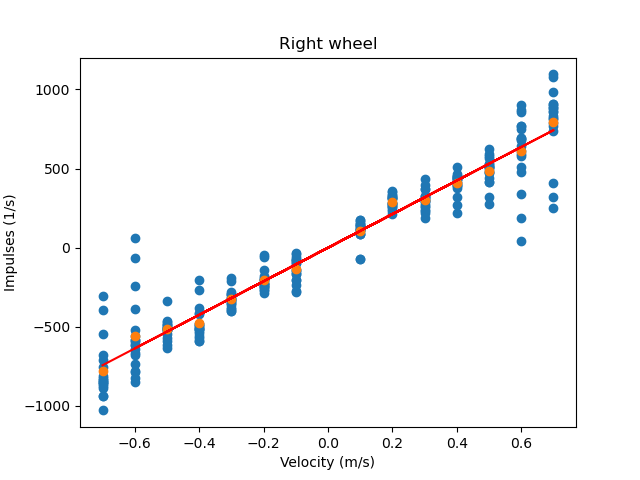
\includegraphics[width=\textwidth]{img/rw_075250.png}
	\end{subfigure}
	\caption{Získanie prevodu z~impulzov na~rýchlosť v~SI jednotkách. \(\alpha\) = 0,75.}
	\label{fig:rw_lw_075250}
\end{figure}

Obr.~\ref{fig:rw_lw_075250} zobrazuje graf výsledkov nameraných pri~aplikácii filtra s~koeficientom alpha o~veľkosti 0,75.
V~tomto prípade sa priemerné hodnoty na~rozdiel od~filtrov s~koeficientami alpha 0,9 a~0,7 dostali takmer priamo na~úsečku
lineárnej regresie prevodu z~impulzov za~sekundu na~metre za~sekundu. Pričom sklon aproximácie sa zmenil pre~ľavý
enkóder na~hodnotu \textbf{1145,83253589} a~pre~pravý enkóder to~je \textbf{1060,25358852}. Použitie silnejšieho filtra
síce pomohlo rýchlejšiemu ustáleniu hodnoty, ale~skúsili sme ešte silnejší filter s~hodnotou alpha $\alpha$ rovnou 0,8.

\begin{figure}[!htbp]
	\begin{subfigure}{0.5\textwidth}
		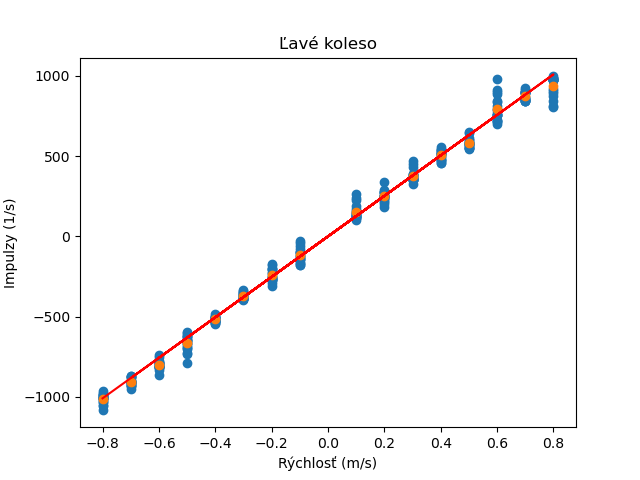
\includegraphics[width=\textwidth]{img/lw_08250.png}
	\end{subfigure}
	\hfill
	\begin{subfigure}{0.5\textwidth}
		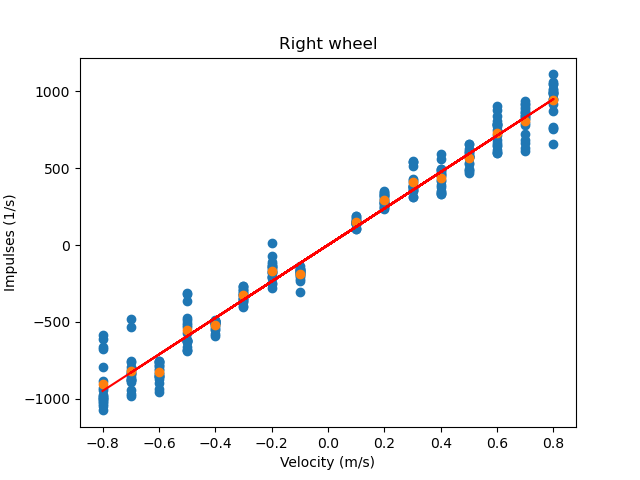
\includegraphics[width=\textwidth]{img/rw_08250.png}
	\end{subfigure}
	\caption{Získanie prevodu z~impulzov na~rýchlosť v~SI jednotkách. $\alpha$ = 0,8.}
	\label{fig:rw_lw_08250}
\end{figure}

Ako môžeme vidieť na~Obr.~\ref{fig:rw_lw_08250} ustálenie hodnôt je veľmi jednoznačné. Vybrali sme si preto~filter s~hodnotou
koeficientu alpha $\alpha$ rovnou 0,8. Zatiaľ všetky dáta čo sme merali boli s~frekvenciou 4Hz (1 vzorka za~250 milisekúnd).
Pre~presnejší výsledok sme túto frekvenciu ešte zvýšili. Z~testov robota sme vypozorovali, že~najfrekventovanejšia frekvencia,
ktorú môže robot sprostredkovať je 10Hz (1 vzorka za~100 milisekúnd). Spravili sme si preto~test na~prevod rýchlosti ešte raz
s~rovnakou hodnotou koeficientu alpha $\alpha$ rovnou 0,8, ale~s~frekvenciou 10Hz namiesto už~spomenutých 4Hz.

\begin{figure}[!htbp]
	\begin{subfigure}{0.5\textwidth}
		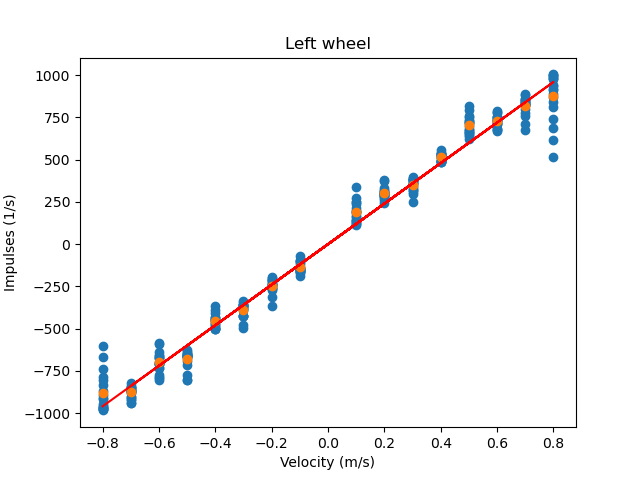
\includegraphics[width=\textwidth]{img/lw_08100.png}
	\end{subfigure}
	\hfill
	\begin{subfigure}{0.5\textwidth}
		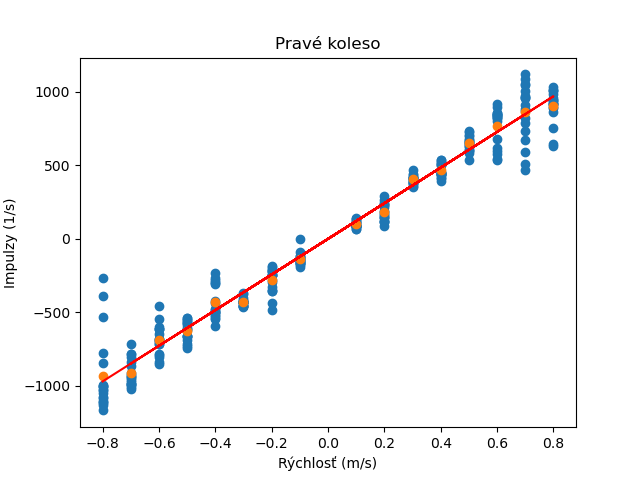
\includegraphics[width=\textwidth]{img/rw_08100.png}
	\end{subfigure}
	\caption{Získanie prevodu z~impulzov na~rýchlosť v~SI jednotkách. $\alpha$ = 0,8 a~frekvenciou 10Hz.}
	\label{fig:rw_lw_08100}
\end{figure}

Najlepšia možná hodnota tohto koeficientu nám vyšla $\alpha$ rovná 0,8. Pri~implementácii tohto filtra sme museli myslieť na~dôležitú vec.
Keď sa zmenia jednorazovo impulzy na~hodnotu 0 a~hneď spať, tak~nám táto vzorka pokazí výsledok. Musíme preto~túto vzorku ignorovať. Ďalšia
prekážka, ktorú sme mali pred sebou bola zmena rýchlosti. Obyčajná implementácia filtra by nám spomalila zmenu vypočítanej rýchlosti
a~teda aj~veľkú odchýlku v~polohe. Tento problém sme opravili prestavením počiatočnej hodnoty filtra na~prvú hodnotu po~zmene rýchlosti.
Toto riešenie sa ukázalo ako najlepšie so~skúšaných riešení.

Problém so~zlou počiatočnou hodnotou môžeme vidieť aj~na~posledom grafe Obr.~\ref{fig:rw_lw_08100_3}. Tento problém sme vyriešili
predpočítavaním prvej hodnoty filtra po~zmene rýchlosti. Keďže sme už~mali koeficienty lineárnej regresie, tak~sme ich využili
na~predpočítanie počiatočnej hodnoty. Výsledok tohto postupu vidíme na~nasledujúcom grafe.

\begin{figure}[!htbp]
	\begin{subfigure}{0.5\textwidth}
		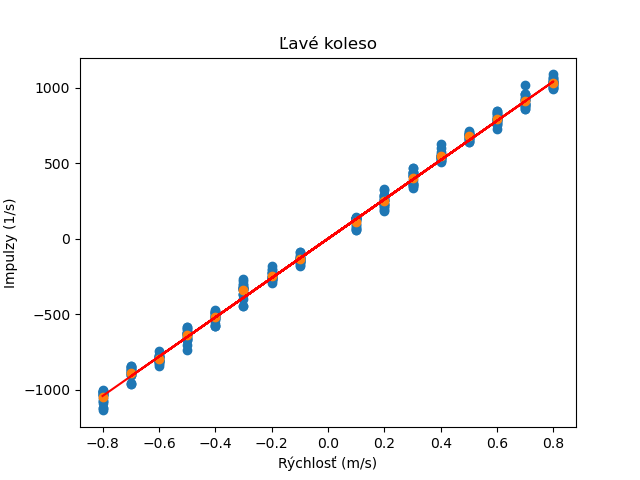
\includegraphics[width=\textwidth]{img/lw_08100_3.png}
	\end{subfigure}
	\hfill
	\begin{subfigure}{0.5\textwidth}
		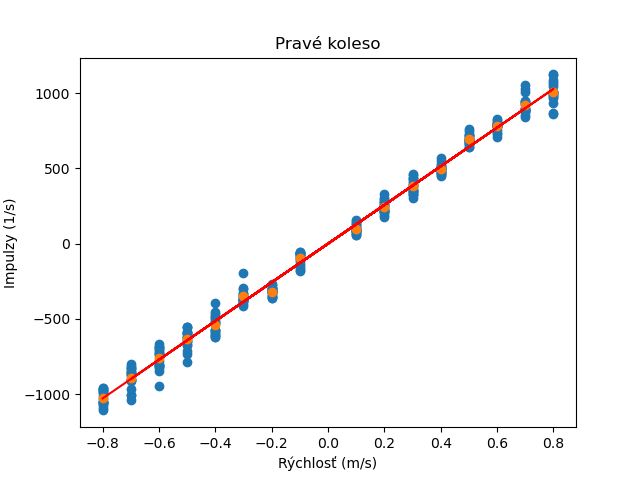
\includegraphics[width=\textwidth]{img/rw_08100_3.png}
	\end{subfigure}
	\caption{Získanie prevodu z~impulzov na~rýchlosť v~SI jednotkách. $\alpha$ = 0,8 a~frekvenciou 10Hz a~prvou prepočítanou hodnotou.}
	\label{fig:rw_lw_08100_3}
\end{figure}

\clearpage

\subsection{Overenie meraní}
\label{subsec:overenie_merani}

Výsledky posledných meraní filtrov sme si vyskúšali na~znázornení prejdenej drahý v~tvare štvorca a~následne sme si
zobrazili na~grafe túto trasu. Pre~porovnanie účinnosti filtra sme porovnali tri grafy. Prvý graf zobrazuje prejdenú
dráhu počas toho ako je filter vypnutý. Druhý graf znázorňuje prejdenú dráhu s~aktívnym filtrom a~jeho hodnota je
najlepšia, ktorú sme namerali. Tretí graf reprezentuje dráhu prejdenú so~silnejším filtrom ako sme sa rozhodli použiť.

\begin{figure}[!htbp]
	\begin{center}
		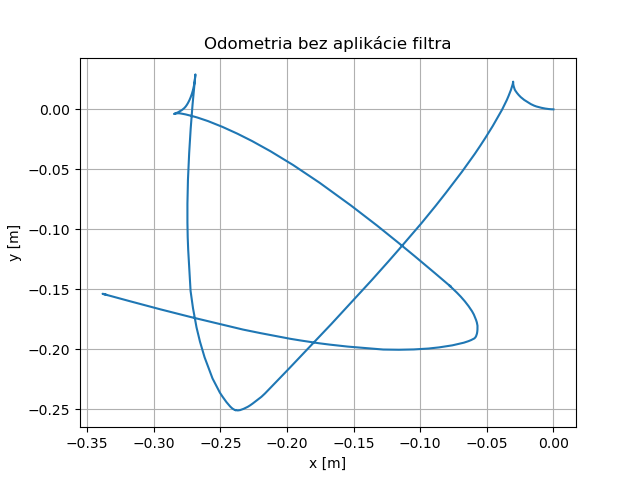
\includegraphics[width=0.8\textwidth]{img/stvorec_bez_filtra.png}
	\end{center}
	\caption{Zobrazenie pohybu robota z~odometrie bez použitia filtra.}
	\label{fig:stvorecBezFiltra}
\end{figure}

Ako prvý pokus sme vypli filtrovanie prichádzajúcich dát. To~malo za~dôsledok, že~všetky skoky, ktoré môžeme vidieť
napríklad na~obrázku Obr.~\ref{fig:rw_lw_nf} sa ukázali na~grafe. Obrázok Obr.~\ref{fig:stvorecBezFiltra} reprezentuje
dráhu, ktorú robot prešiel bez aplikácie filtra. Na~grafe môžeme vidieť zašumenie zbieraných dát z~robota. To sa
zobrazuje najmä v~častiach, keď má robot isť rovno. V~prípade, že filter nepožívame, tak~rovne čiary sa premenia na~čiary
s~natáčaním. To spôsobuje nepresné uvedenie aktuálnej polohy. Tieto nepresnosti sa prejavujú aj pri otáčaní robota.
V prípade, že sa robot má otočiť o 90 stupňov, respektíve o $\frac{\pi}{2}$, tak robot toto otočenie reprezentuje iným
uhlom.

Aby sme videli ako ovplyvňuje filter s~nami navrhnutými parametrami tak~sme spravili ďalšie meranie s~filtrom
s~najlepšími hodnotami. Druhý pokus sme zvolili najlepšiu hodnotu filtra s~koeficientom $\alpha$ rovným 0.8.
Obrázok Obr.~\ref{fig:stvorecSFiltrom} reprezentuje dráhu, ktorú robot prešiel, keď sme na~prichádzajúce dáta
aplikovali tento filter.

\begin{figure}[!htbp]
	\begin{center}
		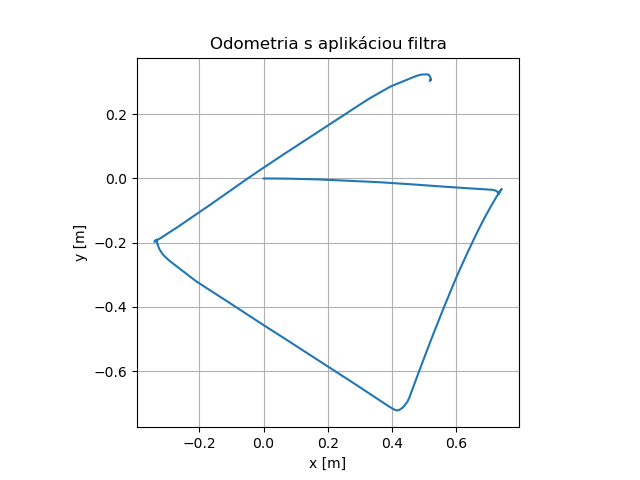
\includegraphics[width=0.8\textwidth]{img/stvorec_s_filtrom_3.png}
	\end{center}
	\caption{Zobrazenie pohybu robota z~odometrie s~použitím najlepšieho filtra.}
	\label{fig:stvorecSFiltrom}
\end{figure}

Ako môžeme vidieť na~tomto grafe tak~síce filter zlepšil výsledok, ktorý sme dostali bez filtra, ale~stále tvar, ktorý
je znázornení na~grafe nie je štvorec. Môže to~byť spôsobené viacerými faktormi.

\begin{itemize}
	\item \textbf{Presmyk} Robot moze na mieste presmukovat. To ma za dosledok nepresne uvedenie polohy robota.
	\item \textbf{Oneskorenie komunikacie} Dáta z ovládača príjmame vo while cykle so softwarovým oneskorením (100ms)
		plus \cite{timovyProjekt}. Tym ze sa moze komunikacia oneskorit, tak to vnasa chybu do vypoctu aktualnej polohy
		na zaklade rychlosti robota.
\end{itemize}

\clearpage

Tretí a~posledný pokus, ktorý sme spravili bolo meranie so~silnejším filtrom ako sme sa rozhodli použiť. Ten
obsahoval koeficient $\alpha$ s~hodnotou 0.9. Pri~takejto konfigurácii filtra sme dostali graf zobrazený
na~obrázku Obr.~\ref{fig:stvorecSoSilnymFiltrom}. Toto zhoršenie spôsobilo zlé zaradenie prijatých impulzov za~sekundu
k~premeneným metrom za~sekundu (Obr.~\ref{fig:rw_lw_09250}).

\begin{figure}[!htbp]
	\begin{center}
		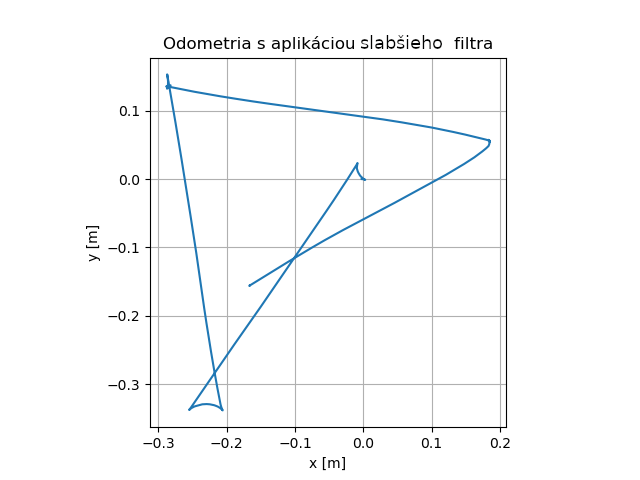
\includegraphics[width=0.8\textwidth]{img/stvorec_so_silnym_filtrom.png}
	\end{center}
	\caption{Zobrazenie pohybu robota z~odometrie s~použitím silnejšieho filtra.}
	\label{fig:stvorecSoSilnymFiltrom}
\end{figure}

